\documentclass[prodmode,acmtecs]{acmsmall} \usepackage[ruled]{algorithm2e}
\usepackage{graphicx}

\acmYear{2015}
\acmMonth{4}

\begin{document}
\title{Accelerating Automated Extraction of Radio Astronomical Sources from Overseation Data with GPU Accelerators
\author{YASEEN HAMDULAY, JARRED DE BEER}
\affil {University of Cape Town}
}

\maketitle{}

\section{Project Description}

Source finding is the detection of galaxies from blind neutral hydrogen surveys of the sky.

Duchamp and Sofia are source finding packages that implement various source finding algorithms.

\subsection{The problem}
MeerKAT and ASKAP are future radio interferometers that are going to survey the sky.
The expected dataset is many orders of magnitude larger than any other dataset we currently have.
We expect our current source finders to take hours to days to run on this data. This is too slow.

\subsection{Why is it important?}
waiting days for source catalogues from source finders is unacceptable. 
This is expensive and wastes the time of the scientists running the experiments. It is a huge
bottleneck and should be cut down.

\subsection{Issues} 
current implementations are too slow
\subsection{difficulties} 
gpu's are difficult to code

\section{Problem Statement}

\subsection{Aim} our aim is to accelerate the process of source finding to the point where it is feasible
to run on meerkat datasets.     

\subsection{Research question} can we accelerate source finding using gpu's?

\subsection{Work division}
Yaseen will implement 2d-1d wavelet reconstruction on the GPU in Duchamp.

Jarred will implement S+C on the GPU in Sofia.

\section{Procedures and Methods}

\subsection{Implementation strategy}
\begin{enumerate}
\item We will reimplement a single threaded version of our algorithm in C/C++.
\item Implement naive GPU version of algorithm in CUDA.
\item Compare two implementations output for correctness
\item Attempt to optimise naive GPU version (using different memory hierarchy strategies)
\end{enumerate}

\subsection{Expected challenges}
\begin{enumerate}
\item Understanding the source finding algorithm from the source code written by the astronomers. 
\item Confirming correcness of source finding implementation.
\item GPU's are difficult to code
\item data dependencies making dividing (and merging) data into subcubes difficult
\item memory bandwidth between GPU and CPU is limited and source finders are memory bandwidth limited (minimising memory congestion).
\item maximising GPU core occupancy.
\item Getting access to GPU cluster in order to test our implementations. 
\item Getting original Sofia and Duchamp creators to integrate our new accelerated algorithms back into sofia and duchamp.
\end{enumerate}

\subsection{Evaluation}
\begin{itemize}
\item We can run the reference implementation (the original found in Duchamp and SoFiA)
on a datacube. Then we run our implementatin on the same data cube and compare the results.
They should be exactly the same.
\end{itemize}

\section{Ethical, professional and legal issues}

SoFiA is GPL version 3.0\\
DUCHAMP is GPL version 2.0\\
We will need to check if re-integrating our code into these repositories will have legal issues with the NRF who is funding our work.

\section{Related Work}
\begin{itemize}
\item A comparison of Source finding algorithms. \cite{popping2012comparison}
\item Parallel Gaussian source finder in OpenCL and CUDA. \cite{westerlund2015performance}
\item K-Means implementation on the GPU. \cite{wu2009clustering}
\item NVidia paper on convolution. \cite{Image Convolution with CUDA by Victor Podlozhnyuk}
\end{itemize}

\section{Anticipated Outcomes}

\subsection{Expected impact}
\begin{itemize}
\item We anticipate the GPU implementation to be considerably faster than the single-threaded implementation. 
\item Faster turn-around time for astronomers when source finding is required.
\end{itemize}

\subsection{Key success factors}
\begin{itemize}
\item Algorithm speed-up.
\item Being merged into the original source finding packages (Sofia and duchamp respectively), 
\item Used in production by astronomers.
\end{itemize}


\section{Project Plan}

\subsection{risks}
\begin{center}
    \begin{tabular}{| p{6cm} | p{0.5cm} | p{6cm} |}
    
    \hline
    Risk & P & Mitigation \\ \hline

    Data format from semi-realistic data cubes is incompatible with
    SoFiA/DUCHAMP packages. & 7 & Convert it to FITS \\ \hline

    Unable to get access to HIPASS data cubes & 6 & Email Paalo Serra and ask for his datacubes \\ \hline

    Algorithm is memory bound to the point where it is unable to be sped up over the CPU. & 6 & Choose another algorithm \\ \hline

    Integrating GPU code with Sofia and Duchamp is infeasible requiring us to
    reimplement key aspects of the source finder framework & 6 & Rewrite input, merging sources etc \\ \hline

    GPU programming is difficult and we may not have sufficient experience to optimise the GPU algorithm
    to the point of achieveing a speedup. & 6 & Consult Chris Laidler, look at Nvidia papers on similar topics, e.g. their convolution paper <cite here> \\ \hline

    The part of the pipeline we choose to implement turns out not to be the bottleneck. & 6 & Profile the execution of the single threaded version before we start implementing it\\ \hline

    A team member drops out of the course.& 6 & Design the implementation strategy such that each member has a similar procedure, but the code, framework and implementation are entirely independent, and can be tested, compiled, integrated individually. Yaseen has chosen DUCHAMP package, Jarred has chosen SoFiA package.\\ \hline

    Processing time takes many hours to complete and power outages become a problem.& 8 & Gain access to UCT's cluster and run it on that\\ \hline
    GPU Kernels take too long to process and are interupted by the Watchdog timer. & 6 & Break the cubes up into smaller subcubes, or write smaller CUDA kernels\\ \hline

    \end{tabular}
\end{center}

\subsection{work allocation diagram}
\begin{figure}
\centerline{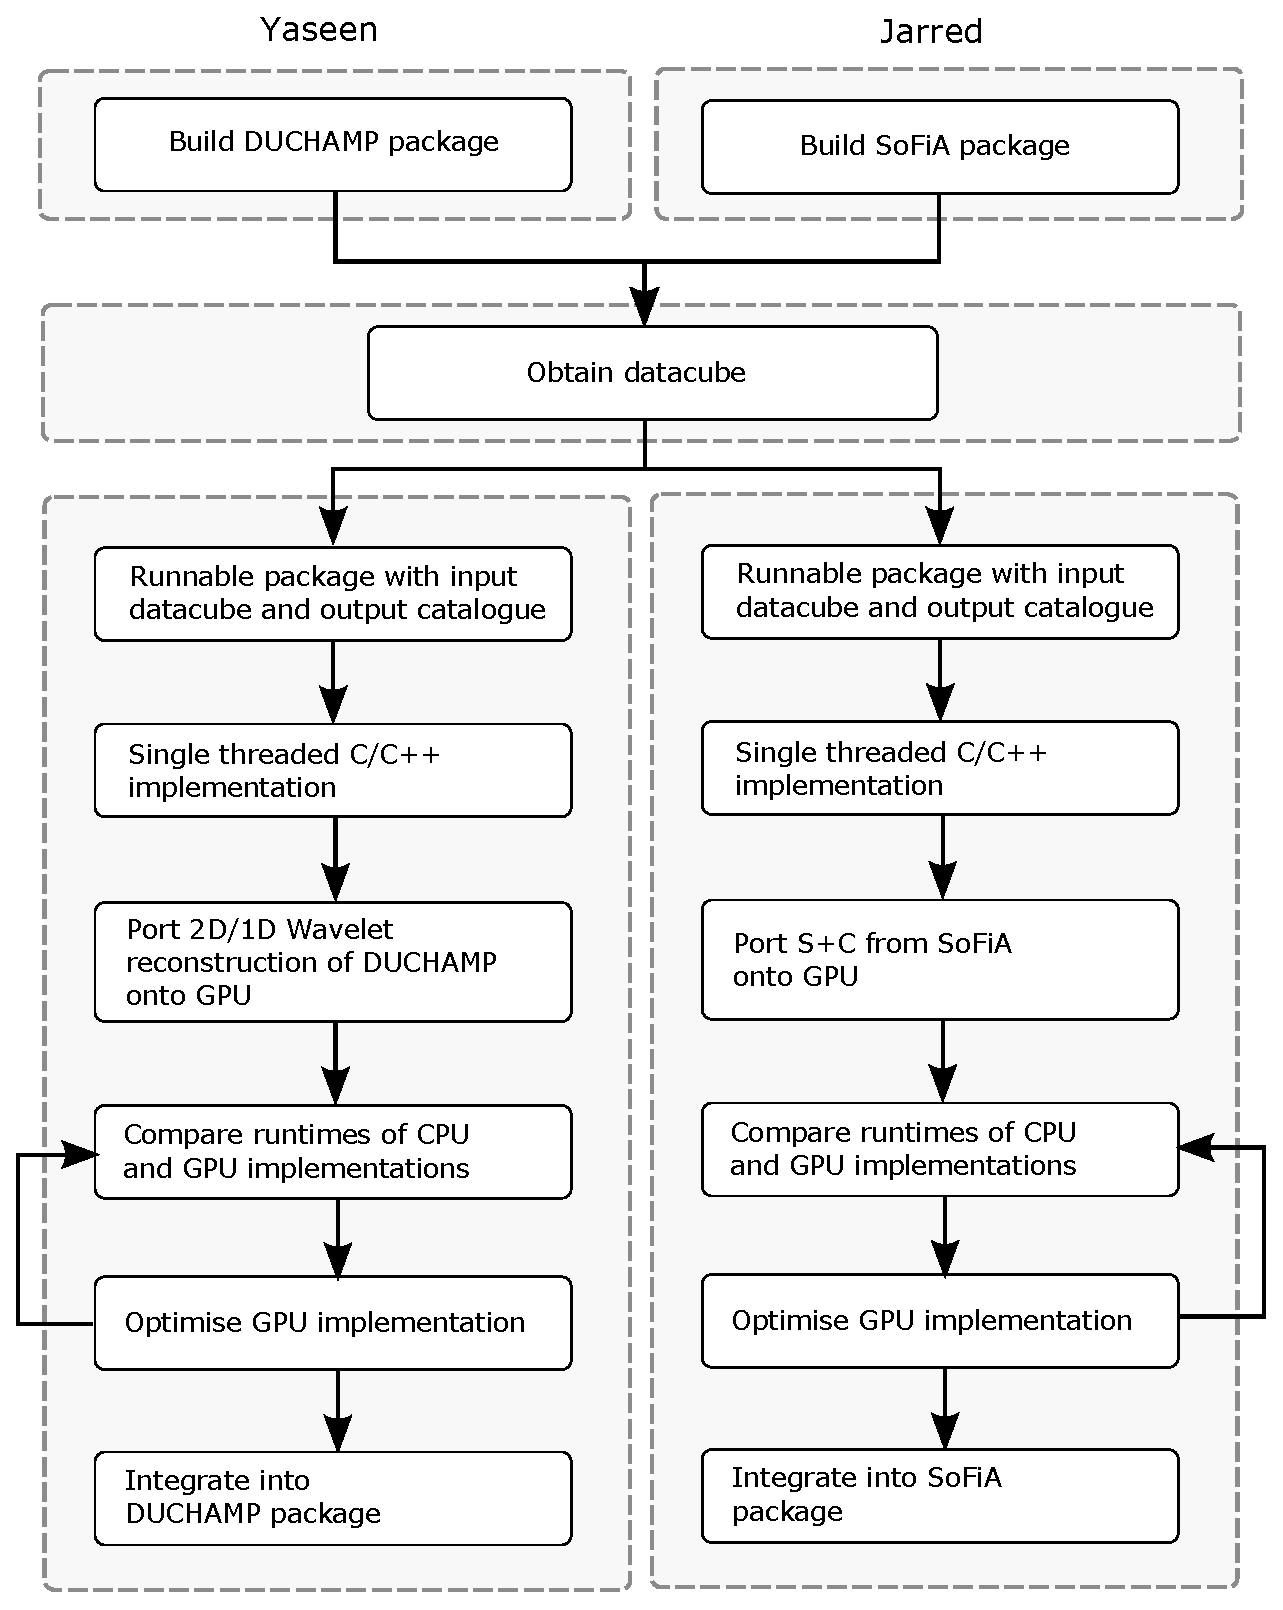
\includegraphics[width=\textwidth,height=\textheight,keepaspectratio]{workallocation}}
\caption{Work allocation between Yaseen and Jarred}
\label{fig:work-allocation}
\end{figure}

\subsection{gantt chart}

\subsection{resources required}
\begin{itemize}
\item Generated semi-realistic data cubes from astronomer.
\item Access to the GPU cluster.
\item HIPASS Parkes All Sky Survey data cubes as well as the catalogues for testing on real data and comparing reliability.
\item Duchamp and Sofia code.
\item NVidia graphics cards for local testing before sending to the cluster.
\end{itemize}

\subsection{deliverables}
\begin{itemize}
\item  Final product with the source finding algorithms integrated into the respective frameworks. Buildable and runnable.
\item  Final report with work completed, our findings and results.
\item  Graphs comparing datacube size with execution time on the original framework implementation, our CPU implementations and GPU implementations.
\end{itemize}

\subsection{milestones}
\begin{itemize}
\item  Have checked out and built the relative packages
\item  Have obtained datacubes and run these against the built packages
\item  Single threaded implementation
\item  Have run performance tests on single threaded implementation
\item  Naive GPU implementation
\item  Have run performance tests on GPU implementation
\item  Optimised GPU implementation
\item  Have run performance tests on Optimised GPU implementation
\item  Have generated graphs from comparison tests
\item  Have integrated our code back into the package source repositories
\end{itemize}

\bibliographystyle{ACM-Reference-Format-Journals}
\bibliography{scaffold}

\end{document}
